\documentclass[draftthesis,tocnosub,noragright, centerchapter,12pt]{uiucecethesis09}

% Use draftthesis for notes and date markings on every page.  Useful when you
%   have multiple copies floating around.
% Use offcenter for the extra .5 inch on the left side. Needed with fullpage and fancy.
% Use mixcasechap for compatibility with hyperref package, which does NOT like all caps default
% Use edeposit for the adviser/committee on the title page.
% Use tocnosub to suppress subsection and lower entries in the TOC.
% PhD candidates use "proquest" for the proquest abstract.

\makeatletter

\usepackage{setspace}
\usepackage{epsfig}  % for figures
\usepackage{graphicx}  % another package that works for figures
\usepackage{subfigure}  % for subfigures
\usepackage{tabularx}
\usepackage{amsmath}  % for math spacing
\usepackage{csvsimple}
\usepackage{subfig}
\usepackage[T1]{fontenc}
\usepackage[font=small,labelfont=bf,tableposition=top]{caption}
\graphicspath{{Images/}}
%\usepackage{amssymb}  % for math spacing
\usepackage{url}  % Hyphenation of URLs.
\usepackage{lscape}  % Useful for wide tables or figures.

\usepackage[justification=raggedright]{caption}	% makes captions ragged right - thanks to Bryce Lobdell

% Uncomment the appropriate one of the following four lines:
\msthesis
%\phdthesis
%\otherdoctorate[abbrev]{Title of Degree}
%\othermasters[abbrev]{Title of Degree}



\title{Multimodal Sentiment Analysis On Songs Using Ensemble Classifiers}
\author{Esteban Gomez}
\department{Electrical and Computer Engineering}
\degreeyear{2015}

% Advi`sor name is required for
% - doctoral students for the ProQuest abstract
% - master's students who do not have a master's committee
\advisor{Minh N. Do}

% Uncomment the \committee command for
% - all doctoral students
% - master's students who have a master's committee
%\committee{Professor Firstname Lastname, Chair\\
%        Professor Firstname Lastname} % etc.

\begin{document}

%%%%%%%%%%%%%%%%%%%%%%%%%%%%%%%%%%%%%%%%%%%%%%%%%%%%%%%%%%%%%%%%%%%%%%%%%%%%%%%
% COPYRIGHT
%
%\copyrightpage
%\blankpage

%%%%%%%%%%%%%%%%%%%%%%%%%%%%%%%%%%%%%%%%%%%%%%%%%%%%%%%%%%%%%%%%%%%%%%%%%%%%%%%
% TITLE
%
\maketitle

%\raggedright
\parindent 1em%

\frontmatter

%%%%%%%%%%%%%%%%%%%%%%%%%%%%%%%%%%%%%%%%%%%%%%%%%%%%%%%%%%%%%%%%%%%%%%%%%%%%%%%
% ABSTRACT
%
\begin{abstract}
% Put the abstract in a file called "abs.tex" and it'll be inputted here.
\title{Multimodal Sentiment Analysis Using Ensemble Classifiers}

We consider the problem of performing sentiment analysis on songs
 by combining audio and lyrics in a large and varied dataset, 
 using the Million Song Dataset for audio features and the 
 MusicXMatch dataset for lyric information. 
 
 The algorithms presented on this thesis utilize ensemble classifiers
  as a method of fusing data vectors from different feature spaces.  
  We find that multimodal classification outperforms using only audio 
  or only lyrics. This thesis argues that utilizing signals from different 
  spaces can account for inter-class inconsistencies and leverages
   class-specific performance. The experimental results show that 
   multimodal classification not only improves overall classification, 
   but is also more consistent across different classes. 
 


Keywords: Music Information Retrieval; Sentiment Analysis; 
Multimodal Classification; Classification Algorithms; Multimodal Fusion

\end{abstract}


%%%%%%%%%%%%%%%%%%%%%%%%%%%%%%%%%%%%%%%%%%%%%%%%%%%%%%%%%%%%%%%%%%%%%%%%%%%%%%%
% DEDICATION
%
%\begin{dedication}
% Whatever dedication you want.
%To my parents, for their love and support.
%\end{dedication}

%%%%%%%%%%%%%%%%%%%%%%%%%%%%%%%%%%%%%%%%%%%%%%%%%%%%%%%%%%%%%%%%%%%%%%%%%%%%%%%
% ACKNOWLEDGMENTS
%
% Put acknowledgments in a file called "ack.tex" and it'll be inputted here.
\begin{acknowledgments}
\title{Acknowldegments}

I want to thank Prof. Minh N. Do, Ben Chidester, and the rest of 
Prof. Minh Do's research group for all the guidance and help they 
have provided through the development of this project.
\end{acknowledgments}

%%%%%%%%%%%%%%%%%%%%%%%%%%%%%%%%%%%%%%%%%%%%%%%%%%%%%%%%%%%%%%%%%%%%%%%%%%%%%%%
% TABLE OF CONTENTS
%
\tableofcontents

%%%%%%%%%%%%%%%%%%%%%%%%%%%%%%%%%%%%%%%%%%%%%%%%%%%%%%%%%%%%%%%%%%%%%%%%%%%%%%%
% LIST OF TABLES
%
% The List of Tables is not strictly necessary. Omitting the List of Tables will
% simplify the thesis check and reduce the number of corrections.
%\listoftables

%%%%%%%%%%%%%%%%%%%%%%%%%%%%%%%%%%%%%%%%%%%%%%%%%%%%%%%%%%%%%%%%%%%%%%%%%%%%%%%
% LIST OF FIGURES
%
% The List of Figures is not strictly necessary. Omitting the List of Figures will
% simplify the thesis check and reduce the number of corrections.
%\listoffigures

%%%%%%%%	%%%%%%%%%%%%%%%%%%%%%%%%%%%%%%%%%%%%%%%%%%%%%%%%%%%%%%%%%%%%%%%%%%%%%%%
% LIST OF ABBREVIATIONS
%!TEX encoding = UTF-8 Unicode
% The List of Abbreviations i	s not strictly necessary.
%\chapter{LIST OF ABBREVIATIONS}

%\begin{symbollist*}
%\item[EPIC] Explicitly Parallel Instruction Computing
%\item[GPU] Graphics Processing Unit
%\item[VLIW] Very Long Instruction Word
%\end{symbollist*}


%%%%%%%%%%%%%%%%%%%%%%%%%%%%%%%%%%%%%%%%%%%%%%%%%%%%%%%%%%%%%%%%%%%%%%%%%%%%%%%
% LIST OF SYMBOLS
%
%\begin{symbollist}[0.7in]
%\item[$\tau$] Time taken to drink one cup of coffee.
%\end{symbollist}

\mainmatter

%%%%%%%%%%%%%%%%%%%%%%%%%%%%%%%%%%%%%%%%%%%%%%%%%%%%%%%%%%%%%%%%%%%%%%%%%%%%%%%
% INSERT REAL CONTENT HERE
%

\renewcommand{\chaptername}{}

\chapter{INTRODUCTION}

In recent years, music-based services have been trying to make their 
applications more user-centered. One way to make sure that the 
user experience is foremost, is to provide services that match the user's 
current emotional state. This can be implemented by understanding 
the emotional content of the songs and playlists that are being played. 

Sentiment analysis is the portion of music informational retrieval (MIR) 
where an algorithm recognizes the main emotions that a song evokes. 
Emotions are subjective, so classifying individual songs into distinct groups 
is a challenging problem. Most human subjects agree in broad 
strokes on emotional classifications. However it is not uncommon
 to find songs where there is no consensus, leading to 
 inconsistencies in class groupings. As a result, sentiment analysis 
 is still an open problem that requires the investigation of alternative methods that 
 employ different modalities to counteract class inconsistencies.  Success in 
 this approach would allow a more robust classification algorithm 
 that is better suited for real-world applications.
  
  The motivation behind this research is to find a method that accounts for 
  these inter-class inconsistencies across a large dataset.  During initial 
  testing it became apparent that certain classifiers perform well on specific 
  sentiments and fail to learn features that represent others. This 
  research seeks to account for this difference by combining the classifiers 
  to output classifications in a  more consistent manner, thus improving the 
  reliability of the overall system.
  
  This thesis will be focusing on the employment of support vector machines (SVM), 
  Gaussian naive bayes and multinomial naive bayes classifiers to recognize
  emotional information.  The audio features that will be employed are based on mel-frequency cepstral coefficients (MFCC),
  which are obtained from the response of the song's windowed spectrogram 
  to a set of basis functions.  A bag-of-words vector is used to represent the lyric portion of the song.  The modal 
  fusion will be tested through both feature fusion and classifier fusion.
  
  The dataset used for this thesis is called the Million Song Dataset, and 
  was compiled by Labrosa \cite{Bertin-Mahieux2011}. This dataset contains a million different songs
  represented by their pitch, loudness, and timbre. The songs are also accompanied 
  by much metadata such as artist, release date, and  tags. Sentiment classification
   was obtained from these tags. If a sentiment was used to describe a song, it is assumed that 
  the song conveyed that sentiment. The lyric information was obtained from the
  MusicXMatch dataset  \cite{musicXmatchDataset}, which provides lyric information out of order in a 
  bag-of-words format. Since there was no way to obtain semantic information 
  from an unordered bag-of-words representation, this research did not focus 
  on the impact of semantics on sentiment classification. 
      
 This report starts with a brief overview of previous work performed on this 
 topic, followed by a description of the methods and the algorithms developed,
 then a section detailing the actual experiments,  a section on results and  analysis.
 It closes with a section on conclusions and suggestions for future work.
 
 \chapter{PREVIOUS WORK}

There has been considerable amount of work done in the field of multimodal 
sentiment analysis. This Chapter will briefly cover a portion of the relevant 
research that was considered during the development of the presented 
methodologies. The relevant topics that were researched for this thesis were: audio sentiment 
analysis, text sentiment analysis, and multimodal classification.


\section*{Audio Sentiment Analysis}

The study of the relationship between emotional content and audio signals is a 
very mature field. Researchers have expanded on the success found in the 
speech recognition community while using mel-frequency cepstral coefficients 
(MFCC) to explore their uses in music modeling \cite{Logan00melfrequency}. MFCCs are currently a 
staple in audio processing and are commonly used in MIR applications such 
as genre classification \cite{Tzanetakis01automaticmusical}, since they are a quantifiable method for comparing the 
timbral texture of songs. Timbre has been used with some success to classify the 
emotional content of songs \cite{University03detectingemotion}; however, class inconsistencies proved to be 
a difficult challenge that creates substantial misclassification between edge cases. 
Timbre has also been used to generate songs that evoke particular emotions \cite{transprose}.  
These vectors have been commonly classified using 
support vector machines (SVM) and naive Bayes classifiers. 

\section*{Text Sentiment Analysis}

Similarly, the study of the relationship between text and emotional content is quite 
developed, applications range from predicting Yelp ratings based on the sentiment expressed on the 
review \cite{YelpReview}  to extracting the emotional progression of major literary pieces \cite{transprose}.  
There are many methods to represent and extract emotional information from texts. 
The Yelp experiment uses statistical word vectors to capture word semantics and 
emotions as a probability.  Other researchers have represented textual information in 
a bag-of-features framework and classified them using naive Bayes, SVMs and 
maximum entropy classifiers to recognize positive or negative valances \cite{Pang:2002:TUS:1118693.1118704}.  

Researchers have extended text processing methods to better capture emotional subtleties. For example, a word can have 
different emotional values depending on its context.  Analyzing this information requires the creation of complex sentiment vectors 
that encode how meanings change based on semantics \cite{Maas:2011:LWV:2002472.2002491}.  Similarly researchers 
have improved classification accuracy by preprocessing text \cite{Haddi201326}, and using the 
cleaned data to capture emotional subtleties like the use of negation and modifiers 
to emotional words \cite{Xia_sentimentvector}. 

Although there is a great body of research on how to obtain rich sentiment vectors 
from text, the goal of this thesis is demonstrate the added advantage of a 
multimodal approach.  For that end, the lyric vectors were kept simple to clearly
underline the benefit of combining them with audio information.  In addition, it is necessary 
to point out that obtaining a large enough dataset of lyrics is difficult due to legal restrictions.   
As a result, the features used will be the unordered representation of the lyrics in 
a bag-of-words vector provided by the MusicXMatch dataset \cite{musicXmatchDataset}.

\section*{Multimodal Classification}

Multimodal classification is the task of using feature vectors from different spaces, 
for example text and audio, to reach a single classification. There are two main 
methods of combining the information from both vector spaces: feature fusion and 
classifier fusion \cite{zhonga2012music}. 

Feature fusion is the technique that takes signals from different 
feature spaces and joins them to train a single multimodal classifier. The standard 
fusion method is called "series fusion", which consists of concatenating the vectors 
together and training the classifier on the union of both spaces. Several alternatives 
have been suggested to maintain the same amount of expressibility in the vector while 
keeping the vector space as small as possible. Instead of concatenating the vectors 
together, it is possible to join vectors in parallel \cite{yang2003feature} by making vectors from the linear
combinations of a real-valued feature with another complex-valued feature. The benefit 
of the series fusion over the parallel method is that many diverse features can be fused
together to obtain more robust data. As seen in the research by Liang et al., 
genre classification was improved by joining five different vectors all resulting from 
different preprocessing methods for text and audio vectors \cite{liang2011music}. 

Classifier fusions train an array of unimodal classifiers and using some 
function to consolidate the predictions \cite{ahmadian2013multi}. This method seamlessly fuses features 
from very different spaces. Caridakis et al. combined facial expressions, body gestures, 
and speech by having a classifier voting system where the class with most votes and 
higher probability was chosen amongst all the decisions \cite{caridakis2007multimodal}. The final decision-making 
process can be taken a step further by adding an additional classifier that learns from 
the decisions provided from classifier array \cite{li2008multi}.  The algorithms presented in this 
research were largely based on this last approach. 


Multimodal classification has been successful in improving the accuracy of classification 
 \cite{zhonga2012music} \cite{hu2010improving}.  However, some of the previous work either ran the experiments on highly homogenous 
datasets where all the music was in the same language, belonged to the same genre, or 
were carefully classified by a single subject thus eliminating class inconsistencies.  The goal of 
this research is to obtain improved classification and reliability from a varied dataset 
through ensemble classifiers. 


	% for INTRODUCTION in "intro.tex"
\renewcommand{\chaptername}{}

\chapter{EXPERIMENT}

Lorem ipsum dolor sit amet, consectetur adipiscing elit. Donec diam dui, posuere non sodales in, consectetur quis magna. Proin dapibus nibh sed turpis sollicitudin, et iaculis massa cursus. Sed interdum metus non arcu interdum hendrerit. Cras eu semper nisi. Etiam hendrerit quam quis ipsum pulvinar, eget commodo augue mattis. Morbi vehicula et ligula in lobortis. Vivamus mattis pharetra tellus eget suscipit. Ut non sem eget diam pharetra efficitur a lacinia quam. Sed ac tempor enim. Nulla facilisi. Ut augue est, sodales eu turpis ut, viverra fringilla sem. Ut sed molestie ex, at rutrum mauris. Donec dignissim dapibus posuere.

Quisque posuere nunc nulla, eget porttitor ligula blandit at. Duis tellus leo, rutrum a massa volutpat, hendrerit euismod nunc. Pellentesque auctor, risus a posuere convallis, velit nulla molestie quam, sit amet viverra sem nulla fermentum nisl. Nulla vel tellus interdum, suscipit diam ac, bibendum erat. Sed a risus ac massa ullamcorper placerat ut ut justo. Nullam faucibus id mi vel vehicula. Nam imperdiet leo ex, pellentesque blandit tellus egestas sed. Nunc pellentesque auctor lacinia. Proin gravida tellus quam. Aliquam erat volutpat. Phasellus hendrerit erat non erat cursus egestas. Ut nec sem quis leo viverra ultricies at nec dolor. Vestibulum ac dictum urna.

Nulla facilisi. Cras vulputate ante ac nisl elementum gravida. Nam quis pellentesque enim. Suspendisse gravida semper turpis at mattis. Aliquam in condimentum nulla, sed molestie enim. Mauris mattis, tortor ut porttitor malesuada, neque urna cursus dui, id sollicitudin nunc velit ut quam. In in turpis at massa auctor egestas at sed neque. Quisque luctus diam in nibh fringilla, vitae iaculis lorem eleifend.  \cite{IEEEexample:book}

Fusce efficitur odio sed magna fermentum congue. In hac habitasse platea dictumst. Pellentesque rhoncus, massa a viverra dapibus, nibh orci euismod dui, eget commodo velit nulla sed lorem. Aenean sed enim eu massa pulvinar venenatis quis vitae odio. Mauris lorem purus, fermentum nec quam gravida, maximus aliquam risus. Mauris ornare justo enim, ut pretium enim lacinia non. Morbi quis pulvinar nibh, in tristique diam. Pellentesque auctor nec diam sed imperdiet. Etiam nec maximus magna. Sed pretium justo in nulla efficitur dictum. Donec maximus nisi vitae est vulputate blandit. Maecenas eget nisi ac odio dignissim pretium. Mauris mollis molestie sapien, eget facilisis urna laoreet ac. Nulla non vulputate risus. Integer sed lacinia tortor. Sed fermentum velit sit amet aliquet efficitur.

Donec vehicula arcu odio, eget pellentesque diam mollis nec. Nam mollis enim eu ultricies sodales. In molestie luctus accumsan. Etiam ut tellus sed elit accumsan dignissim auctor sit amet nulla. Sed augue odio, aliquet a massa et, euismod tempor neque. Ut vitae fringilla lectus. Vestibulum ex lacus, molestie sed viverra non, venenatis sed nulla. Curabitur rutrum enim sapien, et lobortis sapien scelerisque a. Ut faucibus, erat non convallis blandit, dui lorem sollicitudin mauris, sit amet dictum mi enim ac tortor. Integer placerat vehicula tellus vitae egestas.


\chapter{RESULTS}
 
Mauris diam sapien, consequat non velit at, viverra pretium est. Mauris quis leo est. Praesent dictum posuere accumsan. Suspendisse feugiat metus quis risus ultrices, lobortis aliquam purus faucibus. Curabitur viverra tempus massa vitae blandit. Etiam sodales facilisis ullamcorper. Morbi porttitor consectetur est, sit amet vestibulum turpis euismod sagittis. Morbi nec odio nulla. Nunc mollis eros ut velit aliquam mollis. Pellentesque feugiat suscipit nibh, sed consequat eros venenatis at. Quisque nec risus justo. Sed mauris sapien, tincidunt ut dictum a, accumsan faucibus augue. Suspendisse sollicitudin congue arcu, efficitur vulputate nisi semper vitae. Morbi porttitor sodales lorem ac venenatis. Cras vitae tellus ultrices erat ultrices congue posuere ut velit. Quisque id tortor vel arcu efficitur posuere.

Sed molestie nibh lacinia rutrum mattis. Praesent dignissim eget turpis in porta. Fusce ac enim at augue dignissim rhoncus ac quis elit. Etiam accumsan, magna vitae tristique tincidunt, lectus turpis feugiat magna, sit amet consectetur ante risus non erat. In tincidunt ultrices nisl vel dignissim. Phasellus ipsum leo, feugiat et imperdiet nec, cursus et ex. Duis vehicula, sapien ut congue scelerisque, augue leo dictum ex, eget ultricies urna nisi et diam. Aliquam ullamcorper, tellus aliquet bibendum ullamcorper, neque nisl euismod diam, at facilisis ex nisl in leo. Mauris auctor sodales lorem id ultrices. Nullam mauris ligula, sollicitudin at leo et, eleifend tempus ex. Suspendisse nec blandit risus. Suspendisse sollicitudin ipsum vitae orci pulvinar, convallis ullamcorper orci molestie.

Vestibulum egestas dictum eros eu posuere. Vestibulum quis tincidunt sem. Etiam in facilisis dui. Cras viverra magna eget fringilla semper. Etiam ut orci fringilla, faucibus sem ac, facilisis dolor. Nunc molestie, neque id varius fermentum, ipsum sem tempus neque, quis commodo dui tortor placerat nulla. Morbi posuere nisl vitae posuere varius. Phasellus ac accumsan lectus. Nunc dictum fermentum vehicula. Morbi fermentum, odio id sollicitudin sodales, magna nibh vulputate tortor, eget ultricies lacus sem a sem. Quisque pellentesque id libero ac efficitur. Nulla aliquet facilisis venenatis.

Aliquam blandit cursus faucibus. Integer semper est a laoreet tincidunt. Suspendisse potenti. Quisque eget ullamcorper ligula, porta ullamcorper neque. Suspendisse vel justo arcu. Nam pretium turpis id lacinia ultrices. Phasellus ullamcorper lorem est, quis condimentum sem molestie sit amet. Etiam pellentesque sodales ante, vitae rhoncus nisl ornare non. Etiam nec ante laoreet, maximus lectus ac, tempus orci. Proin efficitur ultricies purus, vel volutpat purus ultrices sed. Fusce quis est ex. Nunc suscipit urna et arcu mattis, id vestibulum purus placerat.

Nulla non interdum nulla, vel convallis neque. Praesent eu sapien id tellus convallis bibendum. Integer quis justo et est lacinia consectetur. Praesent nec tellus vitae lacus convallis egestas. Pellentesque aliquam semper quam ut tempor. Sed posuere condimentum arcu, et vulputate nibh sodales ac. Aliquam imperdiet in nulla ac vulputate. Aenean nibh risus, vulputate non risus quis, dignissim pellentesque velit. Donec mi neque, aliquet ut sapien id, lobortis elementum ipsum. Nulla mattis accumsan eros, convallis faucibus ante congue vitae. Nunc pretium ultrices libero. Maecenas eu felis massa.

Donec in enim eget lacus facilisis suscipit. Vestibulum elementum lorem vitae felis euismod tincidunt. Vestibulum ante ipsum primis in faucibus orci luctus et ultrices posuere cubilia Curae; Etiam nec eleifend tellus, ut venenatis metus. Aenean sit amet nisl pellentesque, iaculis purus vel, ornare lorem. Maecenas efficitur porttitor nibh, non malesuada nunc hendrerit ac. Nunc condimentum, orci at porta aliquam, urna purus rutrum mauris, at mattis lorem erat id enim. Nam auctor lacinia neque. Nullam gravida erat sollicitudin, placerat ante a, tincidunt lorem. Lorem ipsum dolor sit amet, consectetur adipiscing elit. In iaculis ipsum nec velit imperdiet, faucibus commodo ipsum tempus.

Cum sociis natoque penatibus et magnis dis parturient montes, nascetur ridiculus mus. Nullam luctus vulputate turpis sit amet gravida. Curabitur id lobortis est, quis pellentesque orci. Cras quis finibus mauris. Curabitur congue elit massa, a pulvinar arcu hendrerit non. Aliquam erat volutpat. Aliquam erat volutpat. In tempor leo ac ex rhoncus, ut facilisis lorem ornare.
\renewcommand{\chaptername}{}

\chapter{RESULTS}
 
This Chapter will present the results of the experiments detailed in the Chapter 4 while providing 
some insight into what differentiates the fusion algorithms from the unimodal benchmarks. To do 
so, two different metrics are used to compare the algorithms. Average accuracy is the standard 
method for comparing classification algorithms. Since one of the goals of this paper is to improve 
the reliability of the overall system in diverse datasets, it is not beneficial to have near perfect 
accuracy for one class and sub-random choice on another class. This gap is smoothed out while 
comparing average accuracies, which is why the algorithms are also compared using  sensitivity.

Sensitivity is a measurement of how well a test recognizes a condition correctly. Sensitivity is only defined 
for binary problems, so the classification outcome had to be reinterpreted to answer the question \lq Does the song belong to this class?'. Since this problem
dealt with three classes, each run created three different one-vs-all confusion matrices for the previous question. Each confusion matrix determined the True Positives (TP) and the False Negatives (FN) for each class, which were used to calculate sensitivity as follows:

\begin{equation}
\text{Sens}_{i} = \frac{TP_i}{TP_i +FN_i} \quad i \in \{\text{happy}, \text{sad}, \text{angry}\}
\end{equation}

The sensibility value assigned to a classifier was the average of all class sensitivities. Since each experiment had thirty runs, then there were a total of ninety different class sensitivities for each classifier. The average of these was considered the classifier's sensitivity.

Table 5.1 contains a summary of the accuracies of all the configurations trained with 500 samples 
for each class. Each row represents an experiment, and it is summarized with the average of all the class accuracies,
 the standard deviation of the class accuracies and the sensitivity mentioned above.  The naming convention used
 to describe each algorithm is as follows: 
 
 \[ \{\text{Method  AudioClassifier - LyricClassifier - MultimodalClassifier}\}  \]  
 
 Where Method can be a unimodal configurations (Audio or Lyrics) or a multimodal configuration 
 ( \lq Full Ensemble',  \lq Audio Partial', \lq Lyric Partial' or \lq Series').
 
\begin{table}
\centering
\footnotesize{
	\hskip-1.0in
	  \caption{Accuracy Measured in Average Accuracy and Sensitivity Using 500 Samples per Class }
	\begin{tabular}{| c | l | c | l | c  ||  c | c | c}\hline%
	& & Average & StdDev & Sensitivity &\pbox{20cm}{ Average\\ Rank \\} & \pbox{20cm}{ Sensitivity\\ Rank \\} \\\hline \csvreader[late after line=\\\hline]%
	{Averages.csv}{Algo=\name,Avg=\avg,Std=\std,Sensitivity=\mte, Rank Average = \ravg, Rank Sens=\rmonte}%
	{\thecsvrow &  \name & \avg & \std & \mte & \ravg & \rmonte}% 
	\end{tabular}
}
\end{table}

\newpage

It is interesting to notice some trends in Table 5.1. First note that the overall accuracy for fusion 
algorithms tends to be slightly higher than the accuracy for the unimodal benchmarks at the 
top of the table.  This is further explored by looking at the standard deviation of these 
accuracies; the benchmarks tend to have a higher variance than the fusion experiments. 
Note that the sensitivity metric tends to be higher when the standard deviation is lower.  
Algorithms with a high sensitivity value tend to do better overall.


Figure 5.1 contains a representation of all the benchmarks and the top two algorithms for each configuration.  One can quickly see that 
series methods do not perform very well. Looking at the other fusion methods, it becomes apparent that doing an initial classification
 of either raw audio or the raw bag of words before fusing the data had drastic benefits.   The best unimodal method is the Lyrics SVM classifier shown in row 7 in Table 5.1. Even
 though it was the best unimodal classifier, it still ranked  $9^{th}$ overall. All algorithms with better ranking are multimodal methods. 

\begin{figure}
\centering
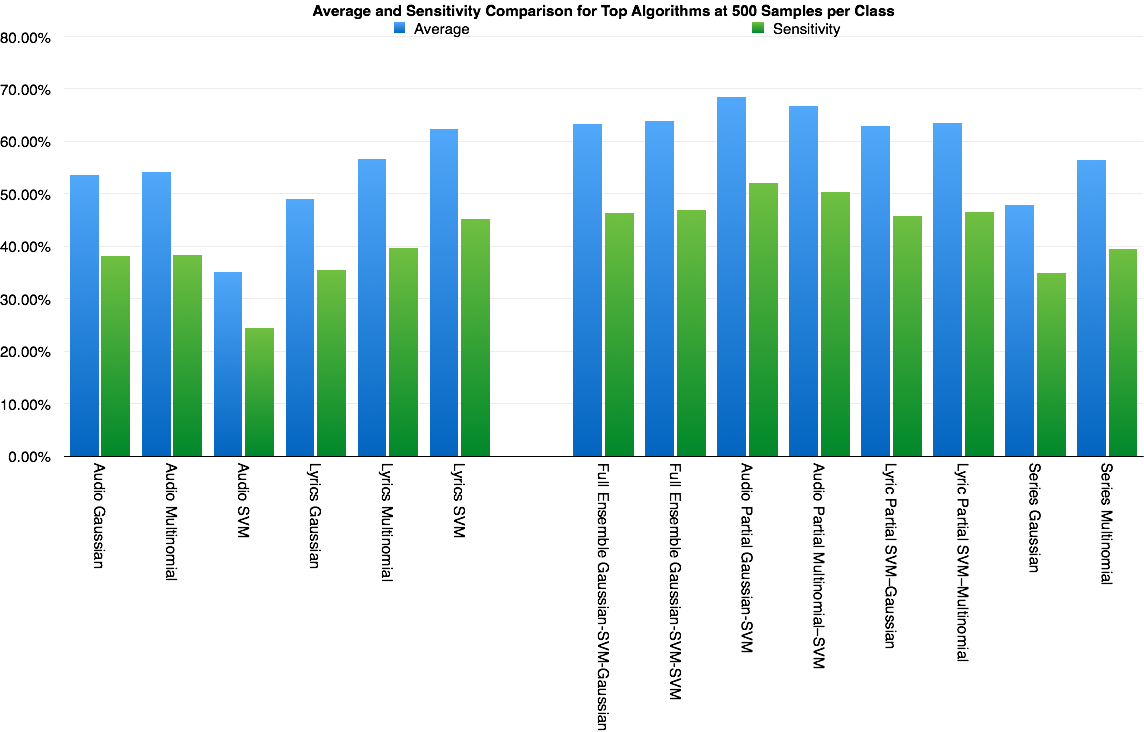
\includegraphics[width=1\textwidth]{Comparison.png}
\caption{Average and Sensitivity Comparison for Top Algorithms at 500 Samples per Class. The left side contains the accuracies and sensitivity values for the unimodal classifiers. The right side contains the accuracies and sensitivity values for the top multimodal classifiers for each configuration.}
\end{figure}

Figure 5.1 shows the performance of the top classifiers and the top benchmarks using 500 training sample per class. 
It provides a good understanding of what configurations are most effective. Figure 5.2 contains the learning curve of some 
of the top classifiers for both unimodal and multimodal. Some of the unimodal classifier perform better at smaller datasets. However once the 
dataset reaches 500 samples per class,  all the multimodal classifiers surpass the unimodal ones. Figure 5.2 also suggests that the training sizes used are not enough
to overfit the data since the slope form most of the curves is increasing for all the points displayed. This behavior indicates that 
a larger dataset should provide better accuracies for many of these algorithms. 


\begin{figure}
 \centering
 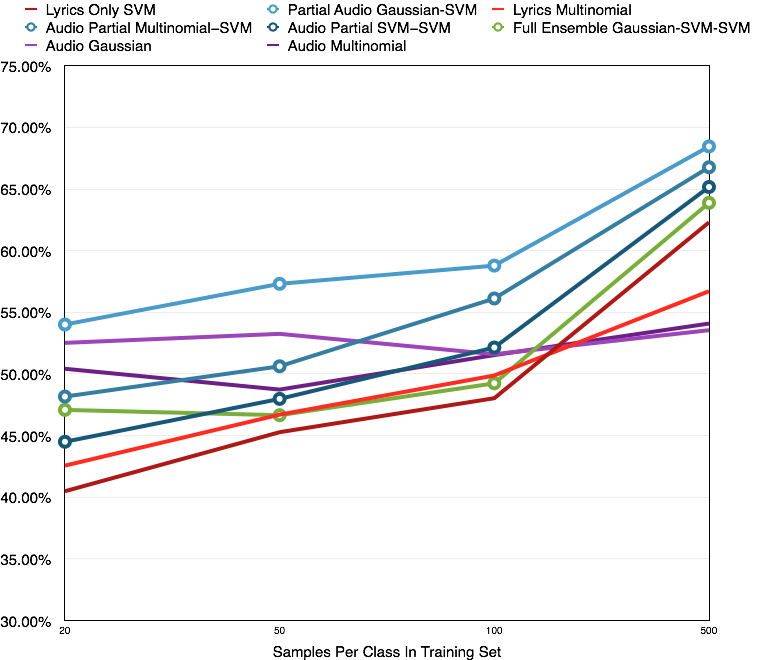
\includegraphics[width=\linewidth]{LearningCurves.png} 
 \caption{Learning Curves for Top Unimodal and Multimodal Classifiers. Plain lines represent unimodal classifiers. While the lines with circles represent the multimodal classifiers. }
\end{figure}

\section*{Better Reliability}

Both the sensitivity and the variance serve as a good indication of the reliability of the system.
A multi-class classification algorithm could possibly have strong average 
recognition accuracy as a result of performing really well for one class but 
poorly for the others.  A high average and a high variance is highly indicative of this case. However,
a high sensitivity or a high average paired with a low variance indicate that the classifier is 
both reliable and accurate. 

Table 5.2 shows the average confusion matrices for the top 
two fusion algorithms and the top three benchmarks. The columns represent 
the true label "H", "S", "A" for the classes happy, sad and angry. The rows 
represent the algorithm's prediction "h", "s", "a" for happy, sad and angry.

Table 5.2 is very informative in terms of what classes are harder to recognize. 
Clearly, happy songs pose a greater challenge than angry songs. This makes 
sense because angry words tend to only be present in angry music. For example 
words like "wrath" or "rage" are more indicative of emotion than words like "sunny" or "cheer".
 The same occurs with the sad classification, but to a lesser extent.
 
 Consider how  the accuracy for angry songs remains relatively constant throughout all the experiments,
but the accuracy for happy songs plummets in Table 5.2.d and Table 5.2.e. Table 5.2.e shows that the audio-only Gaussian 
classifier incorrectly selects the angry classification for 56.77\% of happy songs and for 39.03\% of sad songs. 
 This behavior is evidence that the angry class is getting over-classified, since a disproportionate number of 
 songs receive that classification.  Similarly Table 5.2.d assigns happy songs
 to one of the three classes with almost equal probability, which suggests the classifier cannot identify this class as well as
 others. 
 
These  issues are at play in the case of unimodal classifiers, which would be undesirable for
real world applications. As seen in Table 5.2.a and Figure 5.2.b,  
multimodal classifiers can identify happy songs more accurately without any noticeable loss in angry classification. Both 
 Table 5.2.a and Figure 5.2.b also have a higher accuracy than the best unimodal classifier shown in Table 5.2.c.
Additionally these classifiers do not select a particular class with random chance like Table 5.2.d, nor in a disproportionate manner like Table 5.2.e.




\begin{table}
\centering 
\subfigure[Audio Partial Gaussian-SVM]{
		\begin{tabular}{l |c|c|c|}
			 & H & S & A\\
			\hline
			h & \textbf{58.93\%} & 15.60 \% &16.97\% \\
			\hline
			s & 19.93\% & \textbf{73.07 \%} & 9.67\% \\ 
			\hline
			a & 21.13\% &11.33 \% & \textbf{73.37\%} \\
			\hline
		\end{tabular}
	}
\subfigure[Audio Partial Mutimodal-SVM] {
	\begin{tabular}{l |c|c|c|}
	 & H & S & A\\
	\hline
	h & \textbf{58.70\%} & 19.00 \% &17.80\% \\
	\hline
	s & 18.70\% & \textbf{67.10 \%} & 7.70\% \\ 
	\hline
	a & 22.60\% &13.90 \% & \textbf{74.50} \\
	\hline
	\end{tabular}
}
\subfigure[Lyrics SVM]{
		\begin{tabular}{l |c|c|c|}
			 & H & S & A\\
			\hline
			h & \textbf{52.83\%} & 19.77 \% &17.27\% \\
			\hline
			s & 23.13\% & \textbf{63.93 \%} & 12.60\% \\ 
			\hline
			a & 24.03\% &16.30 \% & \textbf{70.13\%} \\
			\hline
		\end{tabular}
}
\subfigure[Lyrics Multinomial]{

	\begin{tabular}{ l |c|c|c|}
	 & H & S & A\\
	\hline
	h & \textbf{36.93\%} & 13.37 \% &7.87\% \\
	\hline
	s  & 32.23\% & \textbf{59.27 \%} & 18.20\% \\ 
	\hline
	a & 30.83\% &27.37 \% & \textbf{73.93} \\
	\hline
	\end{tabular}
}

\subfigure[Audio Gaussian]{

	\begin{tabular}{ l |c|c|c|}
	 & H & S & A\\
	\hline
	h & \textbf{24.23\%} & 7.80 \% &7.53\% \\
	\hline
	s  & 19.00\% & \textbf{53.17 \%} & 9.20\% \\ 
	\hline
	a & 56.77\% &39.03 \% & \textbf{83.27} \\
	\hline
	\end{tabular}
}

\caption{Confusion Matrices for Top Fusion and Top Benchmarks.  Sub-tables (a) and (b) show that top fusion classifiers are more accurate and reliable than the top unimodal classifier in sub-table (b). Sub-tables (d) and (e) show the most prominent issues found in unimodal classifiers. The column 'H' in sub-tables (d)  shows that the classifier is making random choices to classify the happy class. The row 'a' in table (e) shows that the classifier is over-classifying songs as angry. }
\end{table}


\chapter{Conclusion}

Through the experiments and results presented in this research, we have reached the conclusion that 
multimodal classifiers improve both the accuracy and the robustness of the process.  We 
determined that some sentiments are harder to identify. It was also demonstrated that the recognition of these
challenging sentiments can be improved greatly through multimodal classification without having a significant 
impact on the accuracy of other classes. 


Although many configurations were introduced, the most promising were the \lq Lyric Partial Ensemble' and the \lq Audio Partial
Ensemble'. These two groups dominated the ranks of the top ten in both accuracy and sensitivity. 
All comparison metrics reached the conclusion that the \lq Audio Partial
Ensemble' Audio architecture with an initial Gaussian classifier followed
by an SVM with histogram intersection as a kernel is the strongest classifier explored.



\chapter{FUTURE WORK}
We explored the benefits of combining classification methods in 
different configurations.  The features used for 
the paper underlined the added benefit of multimodal 
classification. Possible future work includes using more complex features that 
take into account sentence semantics to capture word modifiers. Another 
possible route for improvement on this paper would be to extend the number 
of classes used to all six Ekman emotions. 





%%%%%%%%%%%%%%%%%%%%%%%%%%%%%%%%%%%%%%%%%%%%%%%%%%%%%%%%%%%%%%%%%%%%%%%%%%%%%%%
% APPENDIX
%
\appendix
%\include{apx}

\backmatter

%%%%%%%%%%%%%%%%%%%%%%%%%%%%%%%%%%%%%%%%%%%%%%%%%%%%%%%%%%%%%%%%%%%%%%%%%%%%%%%
% BIBLIOGRAPHY
%
\bibliographystyle{IEEE_ECE}
% Put references in BibTeX format in thesisrefs.bib.
\bibliography{thesisrefs}


\end{document}
\endinput
